\documentclass{article} 
\usepackage{graphicx} % Required for inserting images
\usepackage[a4paper, left=2cm, right=2cm, top=2cm, bottom=2cm]{geometry}
\usepackage{tikz}
\usepackage{amsmath, amssymb}
\usepackage{fancyhdr}
\usepackage{helvet} 
\usepackage{lmodern}
\usepackage{booktabs}

\pagestyle{fancy}
\fancyhf{}

\fancyhead[L]{Student : Kuldeep(23684)}  % Left side
\fancyhead[C]{AI-ML (UMC203)}               % Centered
\fancyhead[R]{Instructor : Chiranjib Bhattacharyya}           % Right side

\begin{document}
    \thispagestyle{empty}
    \begin{center}
        \huge{\textbf{Artificial Intelligence and Machine Learning}} \\ 
        \vspace{1cm}
        \huge{\textbf{Assignment 03}} \\ 
        \vspace{2cm}
        \huge{\textbf{Student : Kuldeep Jatav}} \\
        \vspace{0.5cm}
        \huge{\textbf{SR Number: 23684}} \\ 
        \vspace{3cm}

        
\includegraphics[width=0.5\textwidth]{IIScLogo.jpg}
    \end{center}
    
    \newpage
\noindent    \textbf{Q Learning}    

\begin{itemize}
    \item Completed the \texttt{QLAssignment.ipynb} file refer \texttt{23684\_Assignment3.ipynb} attached with this report.
    
    \item I trained the agent  on  two  scenarios,  one  where  traps  and  boots  are  disabled  and another where they are enabled. 
    \begin{itemize}
        \item \textbf{BFS:} The agent is able to reach the goal state in 38 steps using BFS algorithm.
        \begin{figure}[h]
            \centering
            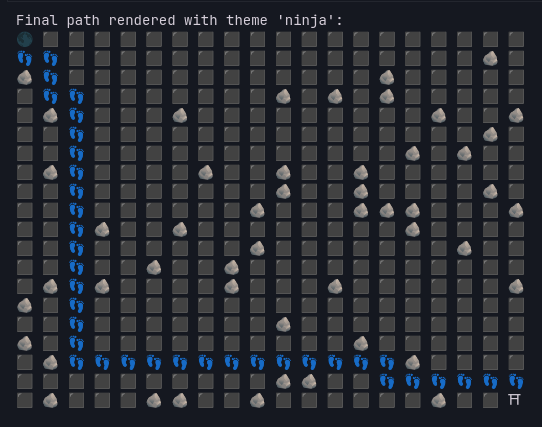
\includegraphics[width=0.45\textwidth]{Path.png}
            \caption{BFS}
            \label{fig:bfs}
        \end{figure}

        \item \textbf{Traps \& Boots:} In both disabled and enabled case the agent took 38 (same as BFS) steps to reach the goal state(see the figure below).  for the configurations 1(mentioned in next part of question).

        \begin{figure}[h]
            \centering
            \begin{minipage}{0.45\textwidth}
                \centering
                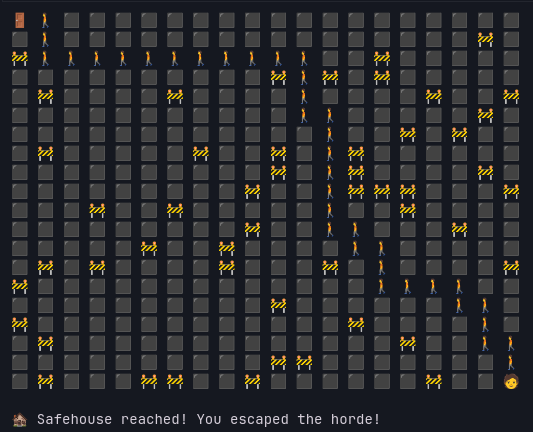
\includegraphics[width=\textwidth]{False.png}
                \caption{Traps and Boots Disabled}
                \label{fig:traps_boots_disabled}
            \end{minipage}
            \hfill
            \begin{minipage}{0.45\textwidth}
                \centering
                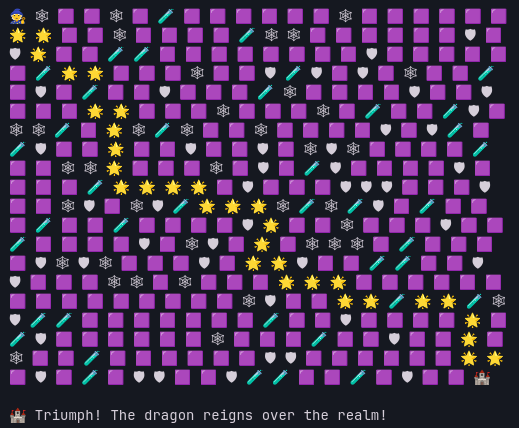
\includegraphics[width=\textwidth]{True.png}
                \caption{Traps and Boots Enabled}
                \label{fig:traps_boots_enabled}
            \end{minipage}
        \end{figure}
    \end{itemize}
    \item \textbf{Different reward configurations:} 

\noindent
    \begin{minipage}{0.6\textwidth}
            \hspace{35pt} \textbf{Configuration 1}
            \begin{itemize}
                \item \texttt{ REWARD\_GOAL = 10000}
                \item \texttt{ REWARD\_TRAP = -500}
                \item \texttt{ REWARD\_OBSTACLE = -100}
                \item \texttt{ REWARD\_REVISIT = -200}
                \item \texttt{ REWARD\_ENEMY = -2000}
                \item \texttt{ REWARD\_STEP = -5}
                \item \texttt{ REWARD\_BOOST = 200}
            \end{itemize}
    \end{minipage}
    \hspace{-20pt}
    \begin{minipage}{0.6\textwidth}
            \hspace{35pt} \textbf{Configuration 2}
            \begin{itemize}
                \item \texttt{ REWARD\_GOAL = 5000}
                \item \texttt{ REWARD\_TRAP = -500}
                \item \texttt{ REWARD\_OBSTACLE = -100   }
                \item \texttt{ REWARD\_REVISIT = -300}
                \item \texttt{ REWARD\_ENEMY = -1500}
                \item \texttt{ REWARD\_STEP = -10 }
                \item \texttt{ REWARD\_BOOST = 250}
            \end{itemize}
    \end{minipage}

\newpage

\hspace{4.5cm} \textbf{Images for configurations 1}

\begin{figure}[h]
    \centering
    \begin{minipage}{0.45\textwidth}
        \centering
        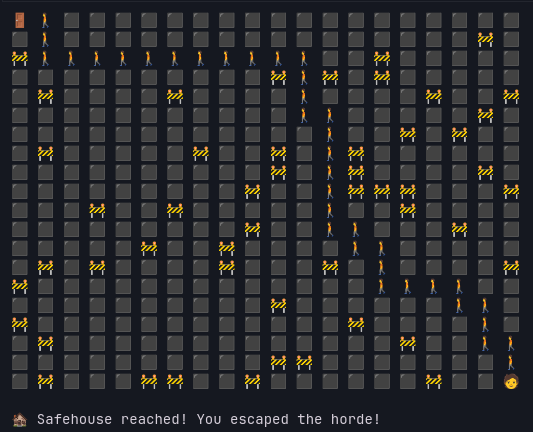
\includegraphics[width=\textwidth]{False.png}
        \caption{Traps and Boots Disabled}
        \label{fig:traps_boots_disabled}
    \end{minipage}
    \hfill
    \begin{minipage}{0.45\textwidth}
        \centering
        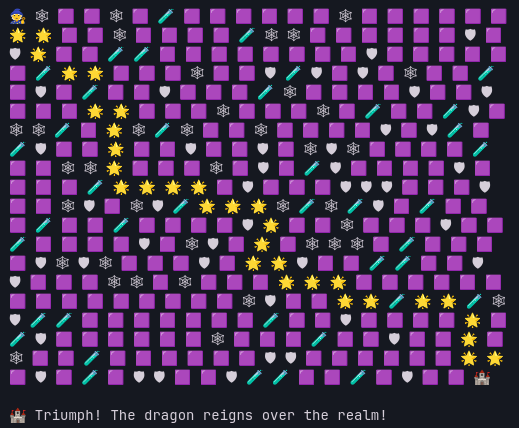
\includegraphics[width=\textwidth]{True.png}
        \caption{Traps and Boots Enabled}
        \label{fig:traps_boots_enabled}
    \end{minipage}
\end{figure}

\hspace{4.5cm} \textbf{Images for configurations 2}

\begin{figure}[h]
    \centering
    \begin{minipage}{0.45\textwidth}
        \centering
        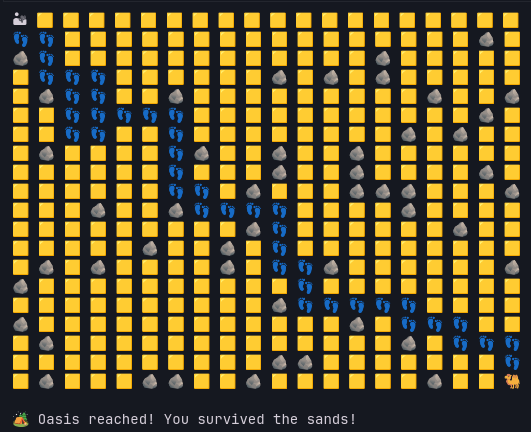
\includegraphics[width=\textwidth]{False2.png}
        \caption{Traps and Boots Disabled}
        \label{fig:traps_boots_disabled}
    \end{minipage}
    \hfill
    \begin{minipage}{0.45\textwidth}
        \centering
        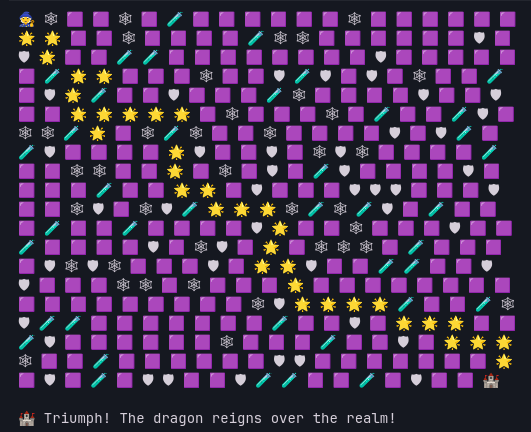
\includegraphics[width=\textwidth]{True2.png}
        \caption{Traps and Boots Enabled}
        \label{fig:traps_boots_enabled}
    \end{minipage}
\end{figure}

\vspace{5pt}

\item \textbf{Manual Q-value Calculation:} For the initial 5 steps, the Q-values are calculated as follows:

\begin{itemize}
    \item \texttt{Learning rate (\(\alpha\)) = 0.4}
    \item \texttt{Discount factor (\(\gamma\)) = 0.95}
    \item Rewards: 
    \begin{itemize}
        \item \texttt{REWARD\_STEP = \(-5\)}
        \item \texttt{REWARD\_GOAL = \(10000\)}
        \item \texttt{REWARD\_OBSTACLE = \(-100\)}
    \end{itemize}
\end{itemize}

We use the Q-learning update rule:
\begin{equation}
    Q(s,a) = Q(s,a) + \alpha \left( r + \gamma \max_{a'} Q(s', a') - Q(s,a) \right)
\end{equation}

\noindent\textbf{Step 1. (0,0) \(\rightarrow\) (1,0)}
\begin{itemize}
    \item Current Q-values for \((0,0)\):
    \begin{tabular}{|c|c|c|c|c|}
        % \hline
        \textbf{Action $\rightarrow$ } & Up & Down & Left & Right \\
        \hline
        \textbf{Q-value $\rightarrow$ } & -767.152172 & -719.833527 & -801.478881 & -631.947255 \\
        % \hline
    \end{tabular}
    \vspace{10pt}
    \item Chosen action: Down (max Q-value = -631.947255)
    \item Reward (\(r\)): \(-5\) (valid move to \((1,0)\))
    \item Next state (\(s'\)): \((1,0)\)
    \item \(\max Q(s', a') = -621.173244\) (from Q-table at \((1,0)\))
    \item Update:
    \begin{align*}
        Q_{\text{new}} &= -631.947255 + 0.4 \left[ -5 + 0.95 \times -621.173244 - (-631.947255) \right] \\
        &= -631.947255 + 0.4 \left[ -5 - 589.1140828 + 631.947255 \right] \\
        &= -631.947255 + 0.4 \times 37.8331722 \\
        &= -631.947255 + 15.13326888 \\
        &= -616.81398612
    \end{align*}
\end{itemize}

\noindent\textbf{Step 2. (1,0) \(\rightarrow\) (1,1)}
\begin{itemize}
    \item Updated Q-values for \((1,0)\):
    \begin{tabular}{|c|c|c|c|c|}
        % \hline
        \textbf{Action $\rightarrow$ } & Up & Down & Left & Right \\
        \hline
        \textbf{Q-value $\rightarrow$ } &-899.367045 & -621.173244 & -725.177182 & -706.806879 \\
        % \hline
    \end{tabular}
    \vspace{10pt}
    \item Chosen action: Right (max Q-value = -621.173244)
    \item Reward (\(r\)): \(-5\) (valid move to \((1,1)\))
    \item Next state (\(s'\)): \((1,1)\)
    \item \(\max Q(s', a') = -650.457508\) (from Q-table at \((1,1)\))
    \item Update:
    \begin{align*}
        Q_{\text{new}} &= -621.173244 + 0.4 \left[ -5 + 0.95 \times -650.457508 - (-621.173244) \right] \\
        &= -621.173244 + 0.4 \left[ -5 - 618.9346326 + 621.173244 \right] \\
        &= -621.173244 + 0.4 \times -2.9613886 \\
        &= -621.173244 - 1.18455544 \\
        &= -622.35779944
    \end{align*}
\end{itemize}

\noindent\textbf{Step 3. (1,1) \(\rightarrow\) (1,2)}
\begin{itemize}
    \item Updated Q-values for \((2,0)\):
    \begin{tabular}{|c|c|c|c|c|}
        % \hline
        \textbf{Action $\rightarrow$ } & Up & Down & Left & Right \\
        \hline
        \textbf{Q-value $\rightarrow$ } & -794.747436 & -650.457508 & -780.813579 & -703.640530\\
        % \hline
    \end{tabular}
    \vspace{10pt}
    \item Chosen action: Right (max Q-value = -650.457508)
    \item Reward (\(r\)): \(-5\) (valid move to \((2,1)\))
    \item Next state (\(s'\)): \((2,1)\)
    \item \(\max Q(s', a') = -634.087470\) (from Q-table at \((2,1)\))
    \item Update:
    \begin{align*}
        Q_{\text{new}} &= -650.457508 + 0.4 \left[ -5 + 0.95 \times -634.087470 - (-650.457508) \right] \\
        &= -650.457508 + 0.4 \left[ -5 - 602.3830965 + 650.457508 \right] \\
        &= -650.457508 + 0.4 \times 43.0744115 \\
        &= -650.457508 + 17.2297646 \\
        &= -633.2277434
    \end{align*}
\end{itemize}

\noindent\textbf{Step 4. (1,2) \(\rightarrow\) (2,2) (Goal)}
\begin{itemize}
    \item Updated Q-values for \((2,1)\):
    \begin{tabular}{|c|c|c|c|c|}
        % \hline
        \textbf{Action $\rightarrow$ } & Up & Down & Left & Right \\
        \hline
        \textbf{Q-value $\rightarrow$ } &-825.636038 & -700.874738 & -791.611875 & -634.087470 \\
        % \hline
    \end{tabular}
    \vspace{10pt}
    \item Chosen action: Right (max Q-value = -634.087470)
    \item Reward (\(r\)): \(-5\) (valid move to \((2,1)\))
    \item Next state (\(s'\)): \((2,1)\)
    \item \(\max Q(s', a') = -618.309086\) (from Q-table at \((2,1)\))
    \item Update:
    \begin{align*}
        Q_{\text{new}} &= -634.087470 + 0.4 \left[ -5 + 0.95 \times -618.309086 - (-634.087470) \right] \\
        &= -634.087470 + 0.4 \left[ -5 - 586.3936317 + 634.087470 \right] \\
        &= -634.087470 + 0.4 \times 42.6938383 \\
        &= -634.087470 + 17.07753532 \\
        &= -617.00993468
    \end{align*}
\end{itemize}

\noindent\textbf{Step 5. (2,2) \(\rightarrow\) (3,2)}
\begin{itemize}
    \item Updated Q-values for \((2,2)\):
    \begin{tabular}{|c|c|c|c|c|}
        % \hline
        \textbf{Action $\rightarrow$ } & Up & Down & Left & Right \\
        \hline
        \textbf{Q-value $\rightarrow$ } &-729.267172 & -661.403121 & -866.272165 & -618.309086 \\
        % \hline
    \end{tabular}
    \vspace{10pt}
    \item Chosen action: Down (max Q-value = -618.309086)
    \item Reward (\(r\)): \(-5\) (valid move to \((3,2)\))
    \item Next state (\(s'\)): \((3,2)\)
    \item \(\max Q(s', a') = -627.114874e\) (from Q-table at \((3,2)\))
    \item Update:
    \begin{align*}
        Q_{\text{new}} &= -618.309086 + 0.4 \left[ -5 + 0.95 \times -627.114874 - (-618.309086) \right] \\
        &= -618.309086 + 0.4 \left[ -5 - 595.7581303 + 618.309086 \right] \\
        &= -618.309086 + 0.4 \times 17.5509557 \\
        &= -618.309086 + 7.02038228 \\
        &= -611.28870372
    \end{align*}
\end{itemize}

\end{itemize}
\hrule
\vspace{4cm}

\begin{center}
    \Huge{\textbf{Thank You}}
\end{center}

\end{document}

